% Practice Test 18 — Virginia Edition
% Questions: 30 (26 MC + 4 SA)
% Generated by scripts/generate_practice_tests.py

\begin{practiceQuestion}{1-4-q12}{mc}
\begin{questionText}
The table shows a proportional relationship. Write the equation and find $y$ when $x = 15$.

\begin{center}
\begin{tabular}{|c|c|}
\hline $x$ & $y$ \\ \hline $2$ & $7$ \\ $4$ & $14$ \\ $6$ & $21$ \\ \hline
\end{tabular}
\end{center}
\end{questionText}
\choiceA{$y = 3.5x$; $y = 52.5$}
\choiceB{$y = 7x$; $y = 105$}
\choiceC{$y = 2x$; $y = 30$}
\choiceD{$y = 3.5x$; $y = 45$}
\correctAnswer{A}
\explanation{$k = \frac{7}{2} = 3.5$. Equation: $y = 3.5x$. When $x = 15$: $y = 3.5 \times 15 = 52.5$.}
\end{practiceQuestion}

\begin{practiceQuestion}{2-1-q04}{mc}
\begin{questionText}
A class has $32$ students. If $75\%$ passed the test, how many students passed?
\end{questionText}
\choiceA{$20$}
\choiceB{$24$}
\choiceC{$25$}
\choiceD{$28$}
\correctAnswer{B}
\explanation{$75\% = 0.75$. Multiply: $0.75 \times 32 = 24$ students passed.}
\end{practiceQuestion}

\begin{practiceQuestion}{2-2-q12}{mc}
\begin{questionText}
Sarah and Jake both solve ``What is $40\%$ of $75$?'' Sarah uses a proportion; Jake uses an equation. Which statement is true?
\end{questionText}
\choiceA{Only the proportion method works}
\choiceB{Only the equation method works}
\choiceC{Both methods give the same answer}
\choiceD{The methods give different answers}
\correctAnswer{C}
\explanation{Proportion: $\frac{n}{75} = \frac{40}{100}$ gives $n = 30$. Equation: $n = 0.40 \times 75 = 30$. Both give $30$.}
\end{practiceQuestion}

\begin{practiceQuestion}{2-3-q12}{mc}
\begin{questionText}
A town's population was $12{,}000$ last year and is $13{,}200$ this year. What is the percent increase?
\end{questionText}
\choiceA{$8\%$}
\choiceB{$10\%$}
\choiceC{$12\%$}
\choiceD{$15\%$}
\correctAnswer{B}
\explanation{Change: $13{,}200 - 12{,}000 = 1{,}200$. Percent increase: $1{,}200 \div 12{,}000 = 0.10 = 10\%$.}
\end{practiceQuestion}

\begin{practiceQuestion}{2-7-q11}{mc}
\begin{questionText}
A carpenter estimated a board was $8$ feet long. The actual length was $8.5$ feet. What is the percent error (rounded to the nearest tenth)?
\end{questionText}
\choiceA{$5\%$}
\choiceB{$5.9\%$}
\choiceC{$6.3\%$}
\choiceD{$6.7\%$}
\correctAnswer{B}
\explanation{$\frac{|8 - 8.5|}{8.5} \times 100 = \frac{0.5}{8.5} \times 100 \approx 5.9\%$.}
\end{practiceQuestion}

\begin{practiceQuestion}{3-2-q02}{mc}
\begin{questionText}
What is $(-12) + 7$?
\end{questionText}
\choiceA{$-19$}
\choiceB{$19$}
\choiceC{$-5$}
\choiceD{$5$}
\correctAnswer{C}
\explanation{Different signs: subtract $12 - 7 = 5$. The larger absolute value is $12$ (negative), so the answer is $-5$.}
\end{practiceQuestion}

\begin{practiceQuestion}{3-3-q13}{mc}
\begin{questionText}
Death Valley's lowest point is $-282$ feet. A nearby hill is $134$ feet above sea level. What is the difference in elevation?
\end{questionText}
\choiceA{$148$ feet}
\choiceB{$-148$ feet}
\choiceC{$416$ feet}
\choiceD{$-416$ feet}
\correctAnswer{C}
\explanation{Difference $= 134 - (-282) = 134 + 282 = 416$ feet.}
\end{practiceQuestion}

\begin{practiceQuestion}{3-4-q03}{mc}
\begin{questionText}
What is $4.2 + (-6.7)$?
\end{questionText}
\choiceA{$10.9$}
\choiceB{$-10.9$}
\choiceC{$2.5$}
\choiceD{$-2.5$}
\correctAnswer{D}
\explanation{Different signs: $6.7 - 4.2 = 2.5$. The larger absolute value ($6.7$) is negative, so the answer is $-2.5$.}
\end{practiceQuestion}

\begin{practiceQuestion}{4-3-q14}{mc}
\begin{questionText}
Which expression is equivalent to $7(a - 3) - 2a$?
\end{questionText}
\choiceA{$5a - 3$}
\choiceB{$5a + 21$}
\choiceC{$9a - 21$}
\choiceD{$5a - 21$}
\correctAnswer{D}
\explanation{Expand: $7a - 21$. Subtract $2a$: $7a - 21 - 2a = 5a - 21$.}
\end{practiceQuestion}

\begin{practiceQuestion}{4-4-q12}{mc}
\begin{questionText}
Factor $20n - 30$.
\end{questionText}
\choiceA{$5(4n - 6)$}
\choiceB{$10(2n - 3)$}
\choiceC{$2(10n - 15)$}
\choiceD{$20(n - 30)$}
\correctAnswer{B}
\explanation{GCF of $20$ and $30$ is $10$. Factor: $20n \div 10 = 2n$ and $-30 \div 10 = -3$. Result: $10(2n - 3)$.}
\end{practiceQuestion}

\begin{practiceQuestion}{5-4-q11}{mc}
\begin{questionText}
Solve $-1.5x + 4.5 = -3$.
\end{questionText}
\choiceA{$x = -5$}
\choiceB{$x = 1$}
\choiceC{$x = 5$}
\choiceD{$x = -1$}
\correctAnswer{C}
\explanation{Subtract $4.5$: $-1.5x = -7.5$. Divide by $-1.5$: $x = 5$. Check: $-1.5(5) + 4.5 = -7.5 + 4.5 = -3$ \checkmark.}
\end{practiceQuestion}

\begin{practiceQuestion}{5-5-q25}{sa}
\begin{questionText}
Solve $-7x - 4 < 17$.
\end{questionText}
\correctAnswer{$x > -3$}
\explanation{Add $4$: $-7x < 21$. Divide by $-7$ and flip: $x > -3$.}
\end{practiceQuestion}

\begin{practiceQuestion}{5-6-q06}{mc}
\begin{questionText}
Solve $-2x \leq 10$ and describe the graph.
\end{questionText}
\choiceA{Closed circle at $-5$, shade left}
\choiceB{Closed circle at $5$, shade left}
\choiceC{Closed circle at $-5$, shade right}
\choiceD{Open circle at $-5$, shade right}
\correctAnswer{C}
\explanation{Divide by $-2$ and flip: $x \geq -5$. Closed circle at $-5$, shade right.}
\end{practiceQuestion}

\begin{practiceQuestion}{6-1-q20}{sa}
\begin{questionText}
A blueprint uses $1$ in $= 9$ ft. A room is $45$ ft long in real life. How long is the room on the blueprint?
\end{questionText}
\correctAnswer{$5$ in}
\explanation{$45 \div 9 = 5$ in.}
\end{practiceQuestion}

\begin{practiceQuestion}{6-2-q14}{mc}
\begin{questionText}
Original scale: $1$ cm $= 10$ m. New scale: $1$ cm $= 40$ m. What is the scale ratio?
\end{questionText}
\choiceA{$\frac{1}{4}$}
\choiceB{$4$}
\choiceC{$30$}
\choiceD{$\frac{1}{30}$}
\correctAnswer{A}
\explanation{Scale ratio: $\frac{10}{40} = \frac{1}{4}$. Every old length is multiplied by $\frac{1}{4}$ on the new drawing.}
\end{practiceQuestion}

\begin{practiceQuestion}{6-5-q17}{mc}
\begin{questionText}
A triangular prism is sliced with a vertical cut perpendicular to the triangular bases. What shape is the cross-section?
\end{questionText}
\choiceA{Triangle}
\choiceB{Rectangle}
\choiceC{Circle}
\choiceD{Trapezoid}
\correctAnswer{B}
\explanation{A vertical cut perpendicular to the triangular bases of a triangular prism produces a rectangle (the cut goes through the lateral faces).}
\end{practiceQuestion}

\begin{practiceQuestion}{6-6-q27}{gmc}
\begin{questionText}
In the diagram below, lines $AB$ and $CD$ intersect at point $O$. Find the value of $y$.

\begin{center}
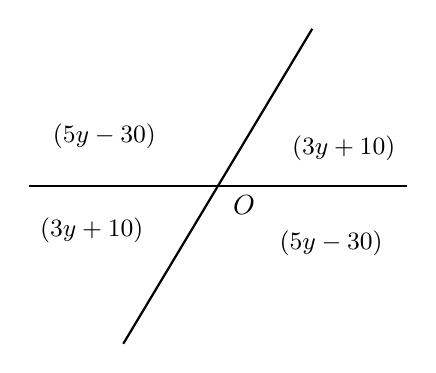
\begin{tikzpicture}[scale=0.8]
  \draw[thick] (-3,0) -- (3,0);
  \draw[thick] (-1.5,-2.5) -- (1.5,2.5);
  \node at (0,0) [below right,xshift=2pt] {$O$};
  \node at (2,0.6) {\small $(3y + 10)°$};
  \node at (-2,-0.7) {\small $(3y + 10)°$};
  \node at (-1.8,0.8) {\small $(5y - 30)°$};
  \node at (1.8,-0.9) {\small $(5y - 30)°$};
\end{tikzpicture}
\end{center}
\end{questionText}
\choiceA{$10$}
\choiceB{$20$}
\choiceC{$25$}
\choiceD{$35$}
\correctAnswer{C}
\explanation{Adjacent angles are supplementary: $(3y + 10) + (5y - 30) = 180$. Combine: $8y - 20 = 180$. Solve: $8y = 200$, $y = 25$.}
\end{practiceQuestion}

\begin{practiceQuestion}{6-7-q09}{mc}
\begin{questionText}
A triangle has vertices $P(1, 2)$, $Q(4, 2)$, and $R(4, 6)$. After a translation, $P' = (3, 0)$. What translation was applied?
\end{questionText}
\choiceA{Right $2$, down $2$}
\choiceB{Left $2$, up $2$}
\choiceC{Right $2$, up $2$}
\choiceD{Left $2$, down $2$}
\correctAnswer{A}
\explanation{From $P(1, 2)$ to $P'(3, 0)$: $x$ changed by $+2$ (right $2$) and $y$ changed by $-2$ (down $2$).}
\end{practiceQuestion}

\begin{practiceQuestion}{6-8-q17}{mc}
\begin{questionText}
A $5$-ft child stands next to a wall that casts a $15$-ft shadow. The child casts a $3$-ft shadow. How tall is the wall?
\end{questionText}
\choiceA{$9$ ft}
\choiceB{$25$ ft}
\choiceC{$45$ ft}
\choiceD{$10$ ft}
\correctAnswer{B}
\explanation{$\frac{5}{3} = \frac{h}{15}$. Cross-multiply: $3h = 75$. Divide: $h = 25$ ft.}
\end{practiceQuestion}

\begin{practiceQuestion}{7-4-q11}{mc}
\begin{questionText}
A T-shaped figure can be broken into a $12$ cm by $2$ cm horizontal rectangle and a $2$ cm by $8$ cm vertical rectangle. What is the total area?
\end{questionText}
\choiceA{$24$ cm$^2$}
\choiceB{$32$ cm$^2$}
\choiceC{$40$ cm$^2$}
\choiceD{$48$ cm$^2$}
\correctAnswer{C}
\explanation{Horizontal: $12 \times 2 = 24$ cm$^2$. Vertical: $2 \times 8 = 16$ cm$^2$. Total: $24 + 16 = 40$ cm$^2$.}
\end{practiceQuestion}

\begin{practiceQuestion}{7-5-q16}{mc}
\begin{questionText}
If all dimensions of a rectangular prism are doubled, what happens to its surface area?
\end{questionText}
\choiceA{It doubles}
\choiceB{It triples}
\choiceC{It quadruples}
\choiceD{It increases by a factor of $8$}
\correctAnswer{C}
\explanation{Surface area depends on the square of the dimensions. Doubling all dimensions multiplies each face area by $2^2 = 4$, so the total surface area quadruples.}
\end{practiceQuestion}

\begin{practiceQuestion}{7-6-q29}{gsa}
\begin{questionText}
A composite solid is made of two rectangular prisms joined together as shown. What is the total volume?

\begin{center}
\begin{tikzpicture}[scale=0.35]
  % Bottom prism
  \draw[thick,funBlue,fill=funBlue!10] (0,0) rectangle (10,3);
  \draw[thick,funBlue,fill=funBlue!20] (10,0) -- (13,2) -- (13,5) -- (10,3) -- cycle;
  \draw[thick,funBlue,fill=funBlue!15] (0,3) -- (3,5) -- (13,5) -- (10,3) -- cycle;
  % Top prism
  \draw[thick,funRed,fill=funRed!10] (0,3) rectangle (4,6);
  \draw[thick,funRed,fill=funRed!20] (4,3) -- (7,5) -- (7,8) -- (4,6) -- cycle;
  \draw[thick,funRed,fill=funRed!15] (0,6) -- (3,8) -- (7,8) -- (4,6) -- cycle;
  % Labels
  \node[below] at (5,0) {$10$ cm};
  \node[left] at (0,1.5) {$3$ cm};
  \node[right] at (13,3.5) {$3$ cm};
  \node[left] at (0,4.5) {$3$ cm};
  \node[above left] at (2,6) {$4$ cm};
  \node[right] at (7,6.5) {$3$ cm};
\end{tikzpicture}
\end{center}
\end{questionText}
\correctAnswer{$126$ cm$^3$}
\explanation{Bottom prism: $10 \times 3 \times 3 = 90$ cm$^3$. Top prism: $4 \times 3 \times 3 = 36$ cm$^3$. Total: $90 + 36 = 126$ cm$^3$.}
\end{practiceQuestion}

\begin{practiceQuestion}{7-7-q18}{mc}
\begin{questionText}
If you double the height of a cylinder but keep the radius the same, what happens to the volume?
\end{questionText}
\choiceA{It stays the same}
\choiceB{It doubles}
\choiceC{It quadruples}
\choiceD{It increases by a factor of $8$}
\correctAnswer{B}
\explanation{$V = \pi r^2 h$. If $h$ becomes $2h$, then $V = \pi r^2(2h) = 2\pi r^2 h$. The volume doubles.}
\end{practiceQuestion}

\begin{practiceQuestion}{8-1-q12}{mc}
\begin{questionText}
Which of the following increases the reliability of conclusions drawn from a sample?
\end{questionText}
\choiceA{Using a smaller sample}
\choiceB{Using a larger random sample}
\choiceC{Surveying only people who agree with you}
\choiceD{Using a non-random sample}
\correctAnswer{B}
\explanation{Larger random samples better represent the population and give more reliable results.}
\end{practiceQuestion}

\begin{practiceQuestion}{8-3-q18}{mc}
\begin{questionText}
School A: median score $88$, MAD $4$. School B: median score $82$, MAD $4$. The difference in medians expressed in MADs is:
\end{questionText}
\choiceA{$1$ MAD}
\choiceB{$1.5$ MADs}
\choiceC{$2$ MADs}
\choiceD{$4$ MADs}
\correctAnswer{B}
\explanation{Difference in medians: $88 - 82 = 6$. In MADs: $\frac{6}{4} = 1.5$ MADs.}
\end{practiceQuestion}

\begin{practiceQuestion}{8-4-q22}{sa}
\begin{questionText}
Group X: mean $45$, MAD $6$. Group Y: mean $57$, MAD $6$. Express the difference in means as a multiple of MAD.
\end{questionText}
\correctAnswer{$2$ MADs}
\explanation{Difference: $57 - 45 = 12$. In MADs: $\frac{12}{6} = 2$.}
\end{practiceQuestion}

\begin{practiceQuestion}{8-5-q18}{mc}
\begin{questionText}
Why is it important to include a key (e.g., ``$3 \mid 4$ means $34$'') in a stem-and-leaf plot?
\end{questionText}
\choiceA{It makes the plot look nicer}
\choiceB{It tells the reader how to interpret the stems and leaves}
\choiceC{It is not important}
\choiceD{It replaces the title}
\correctAnswer{B}
\explanation{The key tells readers what the stems and leaves represent, so they can correctly read the data values.}
\end{practiceQuestion}

\begin{practiceQuestion}{9-3-q03}{mc}
\begin{questionText}
A spinner lands on blue $18$ times out of $90$ spins. What is the experimental probability of landing on blue?
\end{questionText}
\choiceA{$\frac{1}{5}$}
\choiceB{$\frac{1}{4}$}
\choiceC{$\frac{18}{90}$}
\choiceD{Both A and C}
\correctAnswer{D}
\explanation{$P = \frac{18}{90} = \frac{1}{5} = 0.2$. Both A and C represent the same value.}
\end{practiceQuestion}

\begin{practiceQuestion}{9-6-q04}{mc}
\begin{questionText}
Two dice are rolled. What is the probability of getting a sum of $2$?
\end{questionText}
\choiceA{$\frac{1}{6}$}
\choiceB{$\frac{1}{12}$}
\choiceC{$\frac{1}{36}$}
\choiceD{$\frac{2}{36}$}
\correctAnswer{C}
\explanation{The only way to get a sum of $2$ is $(1,1)$. $P = \frac{1}{36}$.}
\end{practiceQuestion}

\begin{practiceQuestion}{9-7-q15}{mc}
\begin{questionText}
You simulate flipping a coin $3$ times and counting how many times all $3$ are heads. In $40$ simulations, all $3$ heads occurs $6$ times. What is the experimental probability?
\end{questionText}
\choiceA{$\frac{6}{40} = 0.15$}
\choiceB{$\frac{1}{8} = 0.125$}
\choiceC{$\frac{3}{40} = 0.075$}
\choiceD{$\frac{6}{120} = 0.05$}
\correctAnswer{A}
\explanation{$P = \frac{6}{40} = 0.15$. The theoretical probability is $\frac{1}{8} = 0.125$, close to the simulation result.}
\end{practiceQuestion}
